\documentclass{article}
\usepackage{booktabs}  % 用于表格 midrule
\usepackage{multirow}  % for multirow command used in the table
\usepackage{amssymb}  % 用于打对号
\usepackage[UTF8]{ctex} % 用于写中文
\usepackage{geometry} % 用于调整页边距
\usepackage{graphicx}  % 用于 includegraphics
\begin{document}
\begin{table}[t]
    \centering
    \caption{Influence of different ways to perturb the search image. The first row demonstrates the the attack performance of the RGB attack method, i.e., the attack attack method proposed in Section III. The second row demonstrates the attack performance of YCbCr attack method: first we convert the search image into YCbCr color space, then add perturbations over the entire search image in the Y channel, and add perturbations over a very small region of $64 \times 64$ in the CbCr channel. The attack performance is evaluated according to AO/SR on GOT-Val.}
    \label{table:random}
    \begin{tabular}{@{}rcccc@{}}
    \toprule
    \multirow{2}{*}[-1pt]{\begin{tabular}[c]{@{}c@{}}Way to perturb\\ the search image\end{tabular}} & \multicolumn{2}{c}{Untargeted Attack} & \multicolumn{2}{c}{Targeted Attack}\\ \cmidrule{2-5}
                                                           & AO                                      & SR                               & AO                & SR                  \\ \midrule
    RGB Attack                                             & 0.246                                   & 0.227                            & 0.682             & 0.756               \\
    RandomAttack                                           & 0.736                                   & 0.871                            & 0.840             & 0.890               \\ \bottomrule        
    \end{tabular}
  \end{table}

\begin{figure}[t]
    \centering
    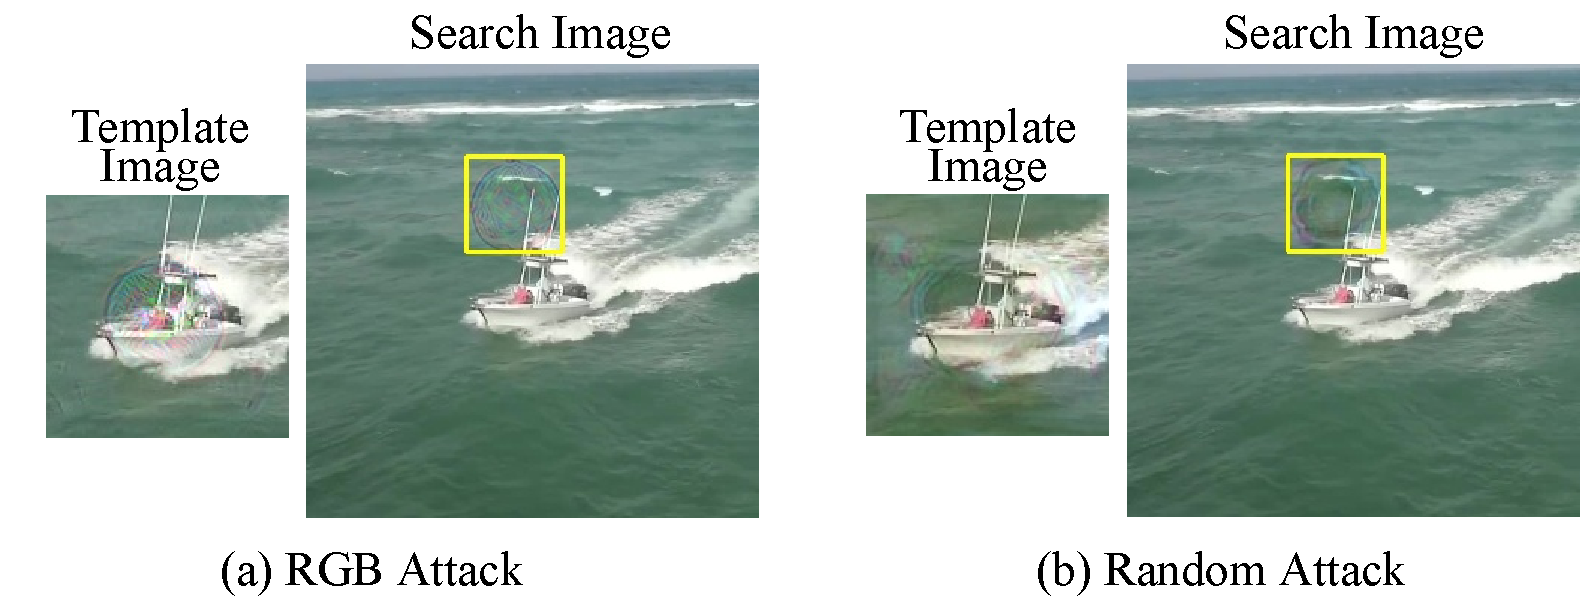
\includegraphics[width=0.8\textwidth]{random.pdf}
    \caption{\uline{Visualization of the perturbations.
    % 介绍什么是 RGB Attack
    Figure (a) demonstrates the pereturbations trained by the RGB attack method, i.e., the attack attack method proposed in Section III.
    % 介绍什么是 YCbCr Attack
    Figure (b) demonstrates the perturbations trained by the YCbCr attack method: first we convert the search image into YCbCr color space, then add pereturbations over the entire search image in the Y channel, and add perturbations over a very small region of $64 \times 64$ in the CbCr channel. 
    For the template image, we convert it into YCbCr color space, then add the perturbation over the entire template image in all YCbCr channels.
    The perturbed template and search images are then converted into RGB color scpace and fed into the tracking network.
    The other steps of the training process are the same as the attack method in Section III.
    Attacking the YCbCr color space brings better imperceptibility. Compared with attacking the RGB space, the SSIM of $p$ increases from 0.56 to 0.78. The SSIM of $\delta$ remains unchanged at 0.79.}
    }
    \label{fig:random}
\end{figure}

Untargeted AO, SR
0.7355267789379769, 0.8707800327017409

targeted AO, SR
0.15291608894028702, 0.11806290276041166

\end{document}